\providecommand{\main}{../..}
\documentclass[../../main]{subfiles}
\usepackage{tikz}
\usetikzlibrary{shapes.geometric, arrows}
\usepackage{longtable}
\begin{document}
\chapter{Facial Expressions}
\label{ch:facial_expressions}

Facial expressions are a crucial element of communication in both spoken and \gls{sl}s. In \gls{sl}s, they serve a dual purpose: conveying the emotional state of the signer and encoding grammatical information such as negation and emphasis. While spoken languages rely on tone and intonation for these functions, \gls{sl}s depend heavily on \gls{non_manual_signals}, particularly facial expressions, to fully convey the meaning of an utterance. Therefore, creating accurate and expressive facial animations in signing avatars is essential for producing realistic and comprehensible \gls{sl} content.

However, synthesizing facial expressions for signing avatars presents significant challenges due to the complexity and subtlety of these expressions. Unlike manual signs, which involve distinct hand and arm movements, facial expressions require the coordinated movement of numerous facial muscles, each contributing to the overall expression. Different facial features, such as eyebrows, eyes, and mouth, often move independently yet in harmony to produce coherent expressions. Previous chapters focused on the synthesis of skeletal features in \gls{sl}. In contrast, this chapter centers on the synthesis of facial expressions from the AZee model, emphasizing their critical role in the conveyance of grammatical information in \gls{sl}s.

The chapter is structured as follows: Section~\ref{ch:facial_expressions:adding_facial_expressions_to_azee} describes the process of extending the AZee model to include facial expressions. Section~\ref{ch:facial_expressions:blendshape_creation} details the creation of blendshapes for facial expressions, while Section~\ref{ch:facial_expressions:motion_curves_for_blendshapes} explains how motion curves are used to animate these blendshapes. Finally, Section~\ref{ch:facial_expressions:results} presents the results of the facial expression synthesis and evaluates the accuracy and expressiveness of the synthesized expressions.

\section{Defining facial expressions in AZee}
\label{ch:facial_expressions:adding_facial_expressions_to_azee}

The AZee model does have a specification for \emph{morph} constraints. However, a proper specification for facial expressions was missing. Thus, our first tasks was to extend the set of \emph{morphs} in the AZee. We used the 40 brèves corpus~\cite{challant2024extending, challant2022first} as a reference for our study. The 40 brèves corpus consists of 23 facial expressions in the form of AZee rules (see section~\ref{annex:facial_expressions:azee_non_manuals} for number of occurrences).

We discussed the \gls{facs} earlier in section~\ref{ch:background_work:sign_language_synthesis:3d_techniques:avatar_animation:face_animation:emotion_recognition}. \gls{facs} is a comprehensive system for describing facial expressions in terms of action units (AUs), which represent the activation of specific facial muscles. AUs can also be combined to create facial expressions. Thus, our first goal is to break down each AZee rule into its constituent AUs. 

We use the AU detector by~\cite{luo2022learning} on mediapipe extractions of still images for each of the facial expressions from the corpus (figure~\ref{ch:facial_expressions:fig:face_detect}).

\begin{figure}[h]
    \centering
    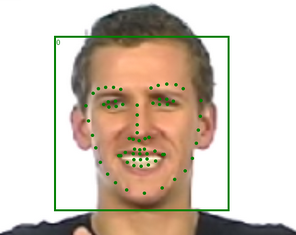
\includegraphics[width=0.8\textwidth]{chapters/facial_expressions/images/face_detect.png}
    \caption{Facial action unit detection using mediapipe and the AU detector by~\cite{luo2022learning} for \emph{big-threatening}}
    \label{ch:facial_expressions:fig:face_detect}
\end{figure}

While it is a good starting point, manual adjustments were required by a linguist to ensure accuracy. This can be seen in figure~\ref{ch:facial_expressions:fig:face_adjust} for the expression \emph{big-threatening}.

\begin{figure}[h!]
    \centering
    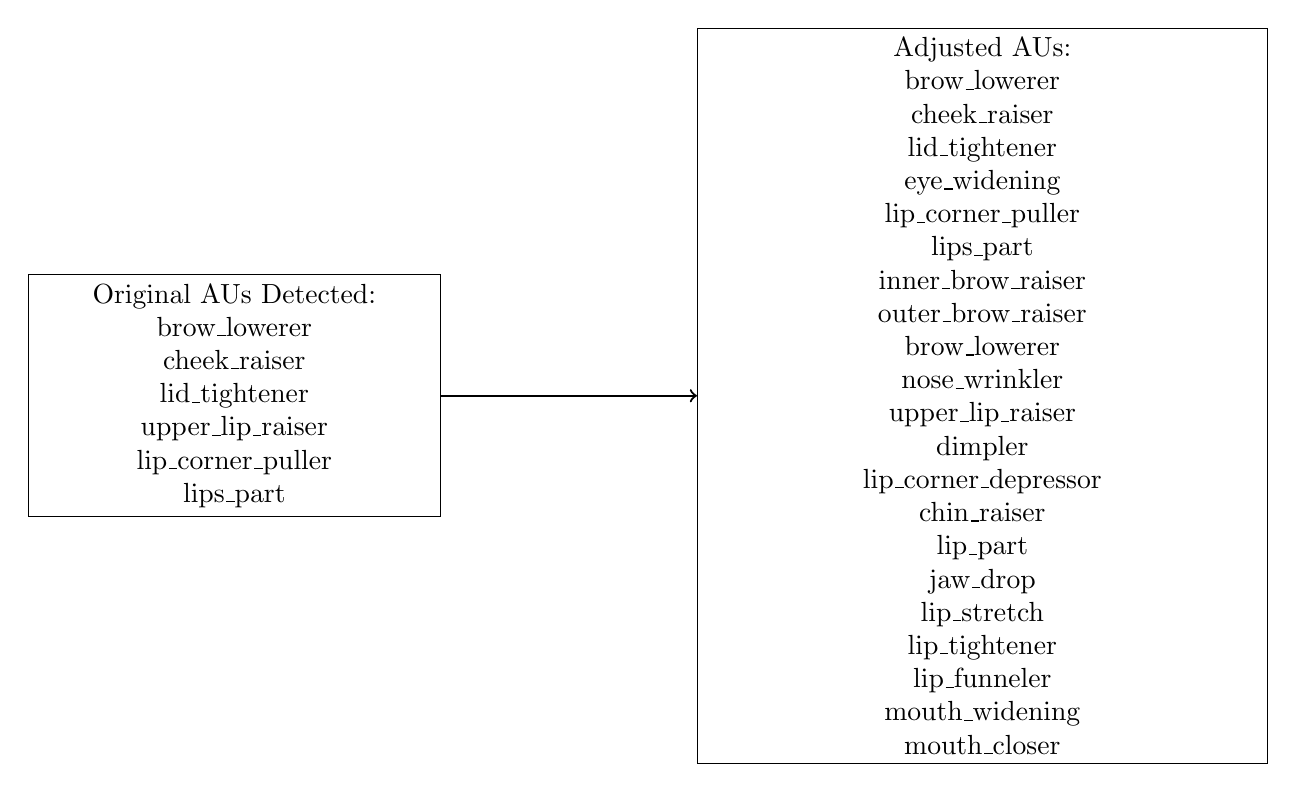
\begin{tikzpicture}[node distance=3.5cm, every node/.style={rectangle, text centered, draw=black}]
    
    % Nodes
    \node (orig) [text width=5cm] {Original AUs Detected: \\ 
      brow\_lowerer \\ 
      cheek\_raiser \\ 
      lid\_tightener \\ 
      upper\_lip\_raiser \\ 
      lip\_corner\_puller \\ 
      lips\_part};
    
    \node (adjusted) [right of=orig, xshift=6cm, text width=7cm] {Adjusted AUs: \\ 
      brow\_lowerer \\ 
      cheek\_raiser \\ 
      lid\_tightener \\ 
      eye\_widening \\ 
      lip\_corner\_puller \\ 
      lips\_part \\ 
      inner\_brow\_raiser \\ 
      outer\_brow\_raiser \\ 
      brow\_lowerer \\ 
      nose\_wrinkler \\ 
      upper\_lip\_raiser \\ 
      dimpler \\ 
      lip\_corner\_depressor \\ 
      chin\_raiser \\ 
      lip\_part \\ 
      jaw\_drop \\ 
      lip\_stretch \\ 
      lip\_tightener \\ 
      lip\_funneler \\ 
      mouth\_widening \\ 
      mouth\_closer};
    
    % Arrows
    \draw[thick,->] (orig) -- (adjusted);
    
    \end{tikzpicture}
    \caption{Manual adjustment for \emph{big-threatening}}
    \label{ch:facial_expressions:fig:face_adjust}
\end{figure}

In total, we extended the low-level AZee language morph set with 94 morphs corresponding to most of the action units in the \gls{facs} system (figure~\ref{tab:added_units}) along with some additional blendshapes for the tongue. A few action units were not added (table~\ref{tab:not_added}) since they were controlled by other skeletal constraints. Some morphs are also alternative blendshapes for the same action units (figure ~\ref{tab:alternative_blendshapes}) but with a different effect on the face.

\section{Modeling Blendshapes for Facial Expressions}
\label{ch:facial_expressions:blendshape_creation}

Once the AUs were identified, we used FACSHuman~\cite{gilbert2021facshuman} blendshapes as reference to create shapekeys on our BAZeel avatar that correspond to each AU (figure~\ref{ch:facial_expressions:fig:facshuman_blendshapes}). Shape keys (figure~\ref{ch:facial_expressions:fig:shape_keys}) are essentially different versions of a 3D model, each representing a specific change in vertices. By blending and interpolating these keys together, we can create a wide range of mesh shapes.

Since the FACSHuman blendshapes work on any MakeHuman template mesh, this technique of synthesis is avatar-independant. However, since the original model did not cover all the blendshapes for every facial mesh, some were created manually. The creation of blendshapes also involved ensuring that they could be seamlessly combined to create complex expressions. For example, the blendshape for AU4 (Brow Lowerer) was designed to work in conjunction with AU6 (Cheek Raiser) and AU12 (Lip Corner Puller) to create expressions of anger or determination.

Let \( V \) be the set of vertices of the 3D facial mesh, where \( V = \{ v_1, v_2, \dots, v_n \} \), and each vertex \( v_i \) has a position in 3D space \( v_i = (x_i, y_i, z_i) \). Each facial Action Unit (AU) \( A_j \) modifies the positions of the vertices based on predefined shape key transformations.

\paragraph{Shape Key Definition}
\label{ch:facial_expressions:blendshape_creation:shape_key_definition}

For each AU \( A_j \), let \( S_j \) be the shape key associated with that AU. \( S_j \) defines a vector of vertex displacements for extreme positions. Specifically, for a vertex \( v_i \), the shape key specifies a displacement \( \Delta v_i^j = (\Delta x_i^j, \Delta y_i^j, \Delta z_i^j) \), where:

\[
\Delta v_i^j = (x_i^j - x_i, y_i^j - y_i, z_i^j - z_i)
\]

Here, \( (x_i^j, y_i^j, z_i^j) \) are the extreme position coordinates of vertex \( v_i \) under AU \( A_j \).

\paragraph{AU Activation}
\label{ch:facial_expressions:blendshape_creation:au_activation}

Let \( \alpha_j \in [0, 1] \) be the activation level of AU \( A_j \), where:
\begin{itemize}
    \item \( \alpha_j = 0 \) means the AU is not activated (neutral position),
    \item \( \alpha_j = 1 \) means the AU is fully activated (extreme position).
\end{itemize}

\paragraph{Vertex Position Update}
\label{ch:facial_expressions:blendshape_creation:vertex_position_update}

For a given activation level \( \alpha_j \), the new position \( v_i' = (x_i', y_i', z_i') \) of vertex \( v_i \) under the influence of AU \( A_j \) is computed as:

\[
v_i' = v_i + \alpha_j \Delta v_i^j
\]

This can be expanded as:
\[
x_i' = x_i + \alpha_j \Delta x_i^j
\]
\[
y_i' = y_i + \alpha_j \Delta y_i^j
\]
\[
z_i' = z_i + \alpha_j \Delta z_i^j
\]

\subsection{Combined Effect of Multiple AUs}
\label{ch:facial_expressions:blendshape_creation:combined_effect_of_multiple_aus}

If multiple AUs \( \{ A_1, A_2, \dots, A_k \} \) are active simultaneously, the final position of vertex \( v_i \) is determined by the weighted sum of the displacements for each AU:

\[
v_i' = v_i + \sum_{j=1}^{k} \alpha_j \Delta v_i^j
\]

\begin{figure}[h]
    \centering
    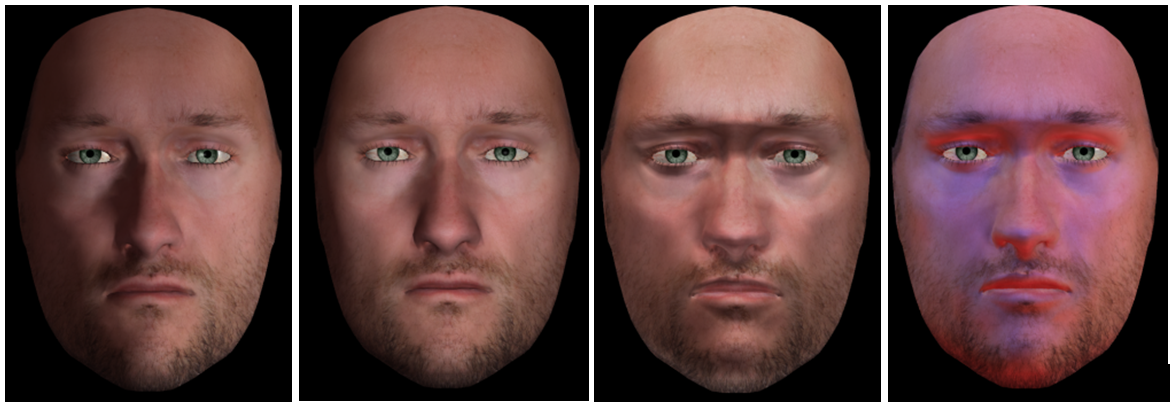
\includegraphics[width=0.8\textwidth]{chapters/facial_expressions/images/facshuman_blendshapes.png}
    \caption{FACSHuman blendshapes used as reference for creating shapekeys in blender.}
    \label{ch:facial_expressions:fig:facshuman_blendshapes}
\end{figure}

\begin{figure}[h]
    \centering
    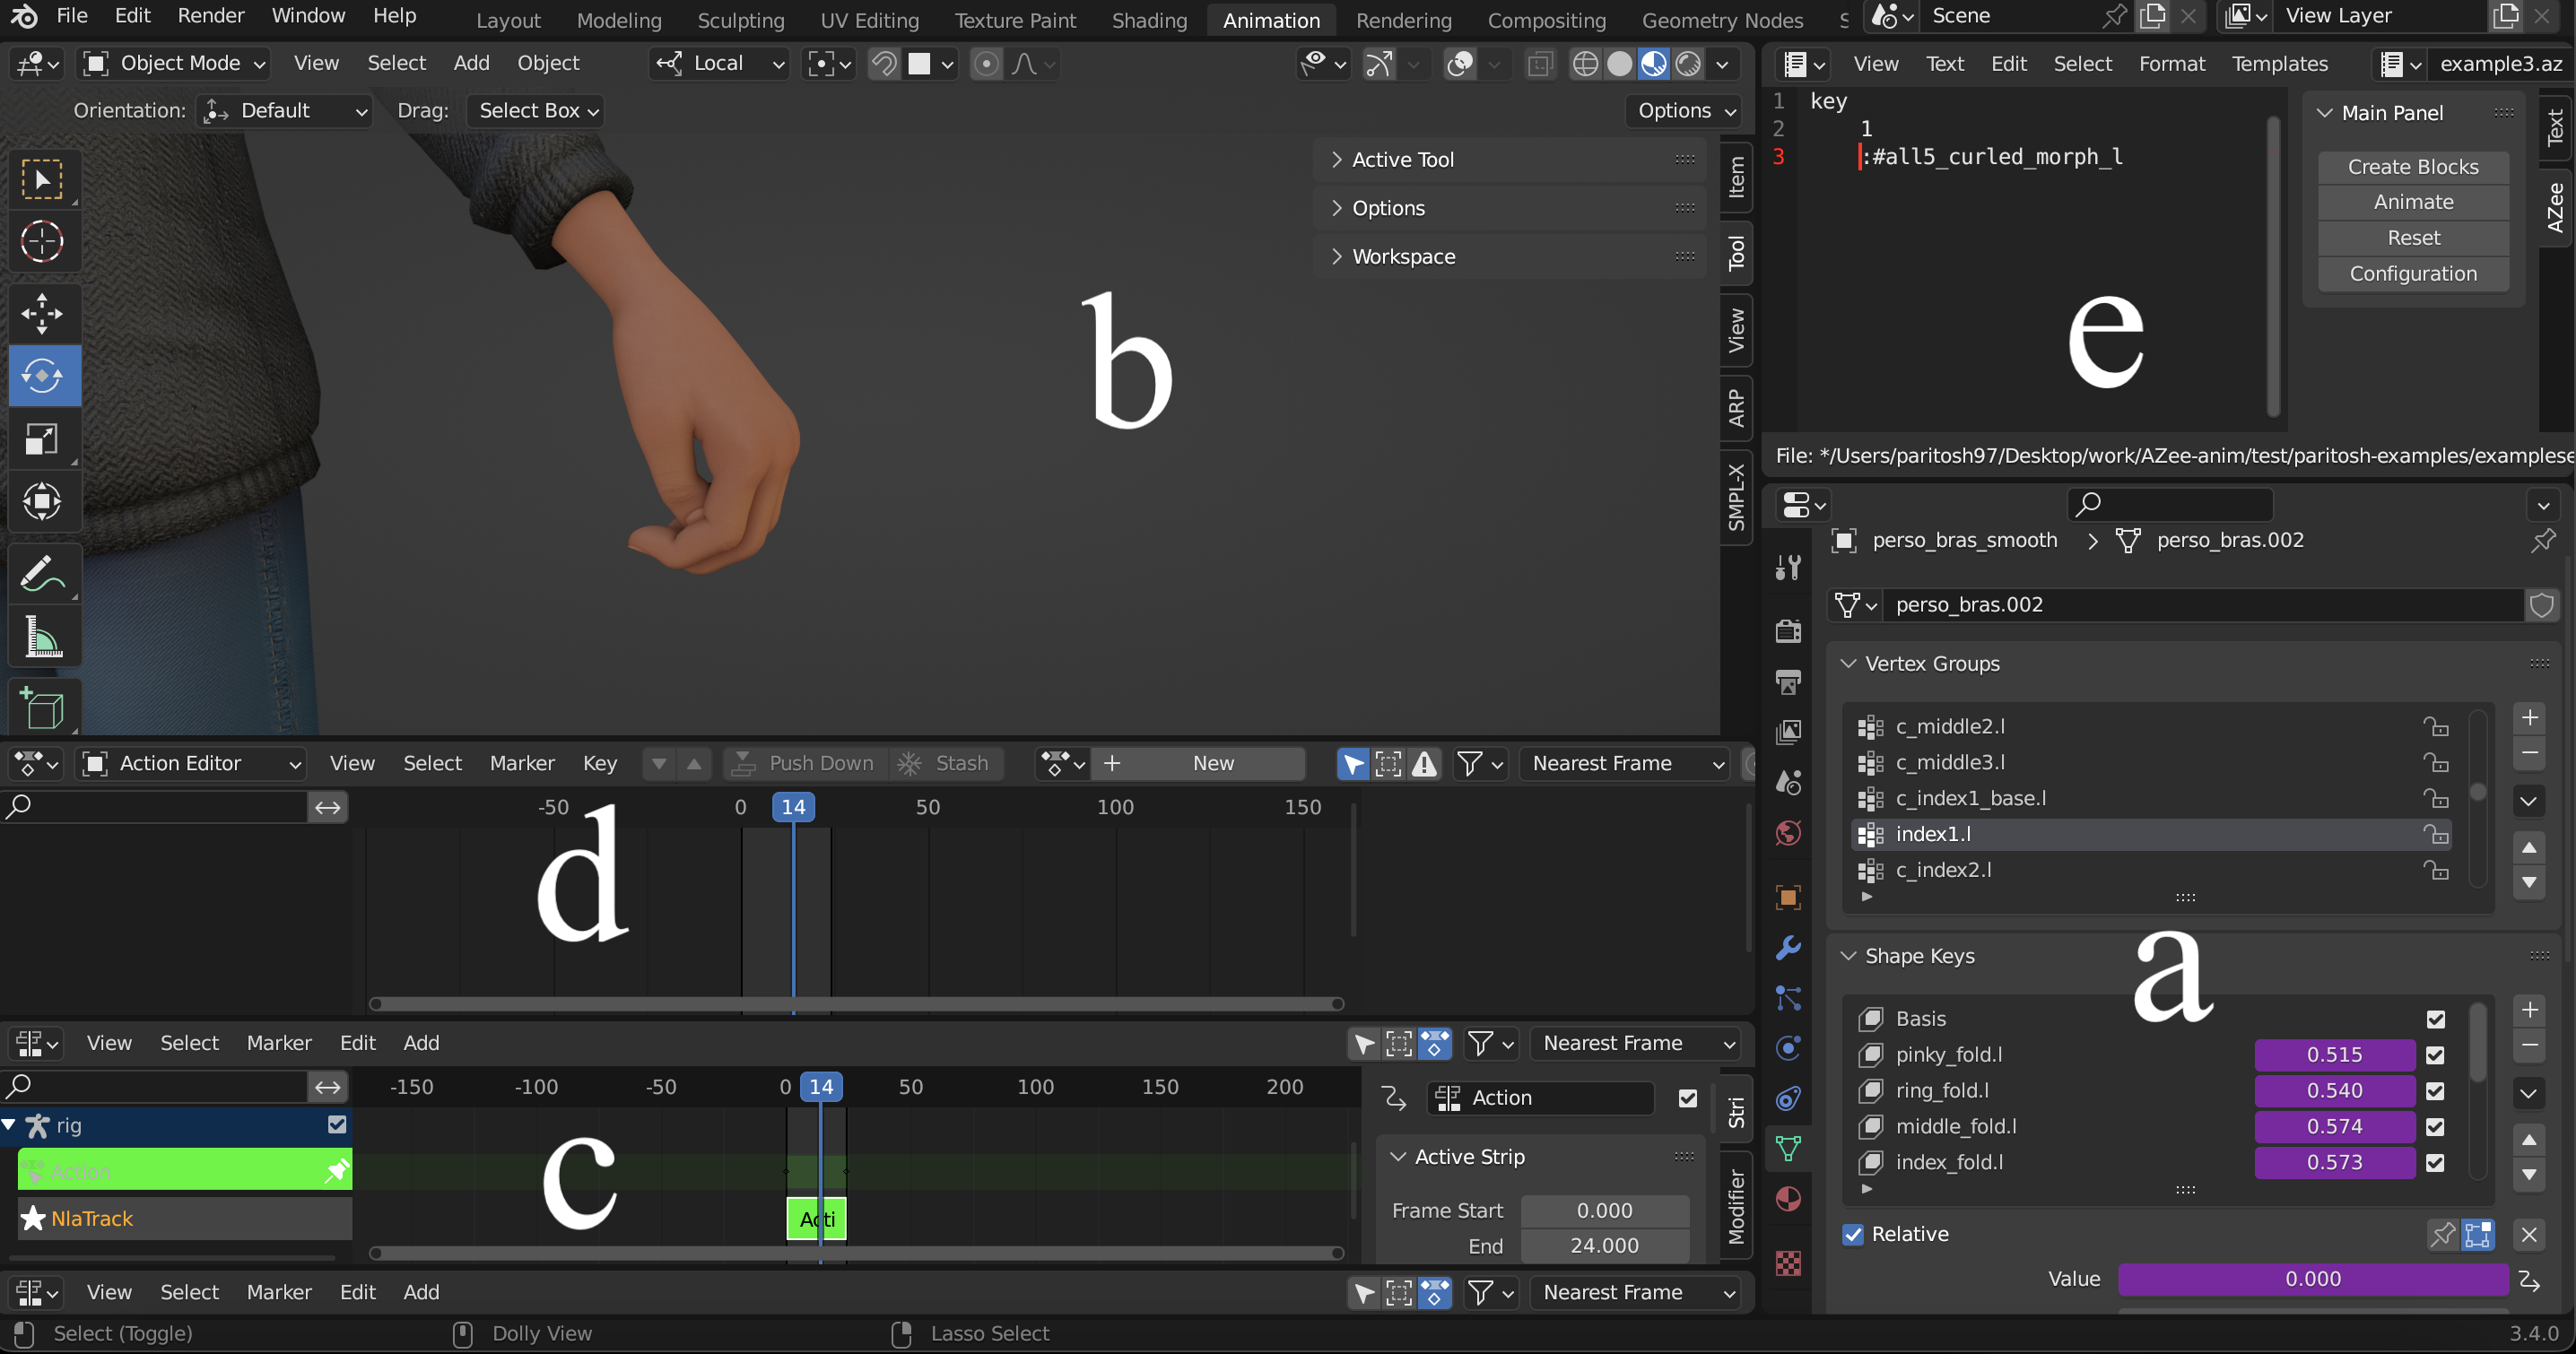
\includegraphics[width=0.8\textwidth]{chapters/facial_expressions/images/shape_keys.png}
    \caption{Blender interface. (a) Shape Key properties (b) 3D Viewport (c) Non-linear Editor (d) Action Editor (e) AZee editor}
    \label{ch:facial_expressions:fig:shape_keys}
\end{figure}

\begin{table}[h]
    \centering
    \scriptsize
    \begin{tabular}{|c|l|c|l|}
        \hline
        \textbf{AU Code} & \textbf{Description}                     & \textbf{AU Code} & \textbf{Description}                      \\ \hline
        AU1              & Inner Brow Raise                        & AU1\_L            & Inner Brow Raise (Left)                   \\ \hline
        AU1\_R           & Inner Brow Raise (Right)                & AU2              & Outer Brow Raise                          \\ \hline
        AU2\_L           & Outer Brow Raise (Left)                 & AU2\_R            & Outer Brow Raise (Right)                  \\ \hline
        AU4              & Brow Lowerer                            & AU5              & Upper Lid Raise                           \\ \hline
        AU5\_L           & Upper Lid Raise (Left)                  & AU5\_R            & Upper Lid Raise (Right)                   \\ \hline
        AU6              & Cheek Raise                             & AU6\_L            & Cheek Raise (Left)                        \\ \hline
        AU6\_R           & Cheek Raise (Right)                     & AU7              & Lids Tight                                \\ \hline
        AU7\_L           & Lids Tight (Left)                       & AU7\_R            & Lids Tight (Right)                        \\ \hline
        AU8              & Lips Toward Each Other                  & AU9              & Nose Wrinkle                              \\ \hline
        AU9\_L           & Nose Wrinkle (Left)                     & AU9\_R            & Nose Wrinkle (Right)                      \\ \hline
        AU10             & Upper Lip Raiser                        & AU10\_L           & Upper Lip Raiser (Left)                   \\ \hline
        AU10\_R          & Upper Lip Raiser (Right)                & AU11             & Nasolabial Furrow Deepener                \\ \hline
        AU11\_L          & Nasolabial Furrow Deepener (Left)       & AU11\_R           & Nasolabial Furrow Deepener (Right)        \\ \hline
        AU12             & Lip Corner Puller                       & AU12\_L           & Lip Corner Puller (Left)                  \\ \hline
        AU12\_R          & Lip Corner Puller (Right)               & AU13             & Sharp Lip Puller                          \\ \hline
        AU13\_L          & Sharp Lip Puller (Left)                 & AU13\_R           & Sharp Lip Puller (Right)                  \\ \hline
        AU14             & Dimpler                                 & AU14\_L           & Dimpler (Left)                            \\ \hline
        AU14\_R          & Dimpler (Right)                         & AU15             & Lip Corner Depressor                      \\ \hline
        AU15\_L          & Lip Corner Depressor (Left)             & AU15\_R           & Lip Corner Depressor (Right)              \\ \hline
        AU16             & Lower Lip Depress                       & AU17             & Chin Raiser                               \\ \hline
        AU18             & Lip Pucker                              & AU19             & Tongue Show                               \\ \hline
        AU20             & Lip Stretch                             & AU20\_L           & Lip Stretch (Left)                        \\ \hline
        AU20\_R          & Lip Stretch (Right)                     & AU21             & Neck Tightener                            \\ \hline
        AU22\_25\_up\_down & Lip Funneler (Both Lips) & AU23             & Lip Tightener                             \\ \hline
        AU24             & Lip Presser                             & AU25             & Lips Part                                 \\ \hline
        AU25\_L          & Lips Part (Left)                        & AU25\_R           & Lips Part (Right)                         \\ \hline
        AU26             & Jaw Drop                                & AU27             & Mouth Stretch                             \\ \hline
        AU28             & Lips Suck                               & AU29             & Jaw Thrust                                \\ \hline
        AU30\_L          & Jaw Sideways (Left)                     & AU30\_R           & Jaw Sideways (Right)                      \\ \hline
        AU31             & Jaw Clencher                            & AU32             & Bite                                      \\ \hline
        AU33             & Blow                                    & AU34             & Puff                                      \\ \hline
        AU35             & Cheek Suck                              & AU36             & Tongue Bulge                              \\ \hline
        AU37             & Lip Wipe                                & AU38             & Nostril Dilate                            \\ \hline
        AU39             & Nostril Compress                        & AU43             & Eye Closure                               \\ \hline
        AU43\_L          & Eye Close (Left)                        & AU43\_R           & Eye Close (Right)                         \\ \hline
    \end{tabular}
    \caption{Added blend shapes} 
    \label{tab:added_units} 
\end{table}

\begin{table}[h]
    \centering
    \scriptsize
    \begin{tabular}{|c|l|c|l|}
        \hline
        \textbf{AU Code} & \textbf{Description}                     & \textbf{AU Code} & \textbf{Description}                      \\ \hline
        AU40             & Sniff                                   & AU41             & Lid Droop                                 \\ \hline
        AU42             & Slit                                    & AU44             & Squint                                    \\ \hline
        AU45             & Blink                                   & AU46             & Wink                                      \\ \hline
        AU51             & Head Turn Left (IK controlled)          & AU52             & Head Turn Right (IK controlled)           \\ \hline
        AU53             & Head Up (IK controlled)                 & AU54             & Head Down (IK controlled)                 \\ \hline
        AU55             & Head Tilt Left (IK controlled)          & AU56             & Head Tilt Right (IK controlled)           \\ \hline
        AU57             & Head Forward (IK controlled)            & AU58             & Head Back (IK controlled)                 \\ \hline
        AU61             & Eyes Turn Left (lookat constraint)      & AU62             & Eyes Turn Right (lookat constraint)       \\ \hline
        AU63             & Eyes Up (lookat constraint)             & AU64             & Eyes Down (lookat constraint)             \\ \hline
    \end{tabular}
    \caption{Action units skipped} 
    \label{tab:not_added} 
\end{table}

\vspace{1cm}

\begin{table}[h]
    \centering
    \scriptsize
    \begin{tabular}{|c|l|c|l|}
        \hline
        \textbf{AU Code} & \textbf{Description}                     & \textbf{AU Code} & \textbf{Description}                      \\ \hline
        AU1\_a            & Inner Brow Raise (Alternative)          & AU2\_a            & Outer Brow Raise (Alternative)           \\ \hline
        AU4\_a            & Brow Lowerer (Alternative A)            & AU4\_b            & Brow Lowerer (Alternative B)             \\ \hline
        AU6\_a            & Cheek Raise (Alternative A)             & AU6\_b            & Cheek Raise (Alternative B)              \\ \hline
        AU9\_a            & Nose Wrinkle (Alternative A)            & AU12\_a           & Lip Corner Puller (Alternative A)        \\ \hline
        AU12\_b           & Lip Corner Puller (Alternative B)       & AU17\_a           & Chin Raiser (Alternative A)              \\ \hline
        AU18\_a           & Lip Pucker (Alternative)                & AU25\_a           & Lips Part (Alternative A)                \\ \hline
        AU22\_25\_upper  & Lip Funneler (Upper Lip)     & AU22\_25\_down   & Lip Funneler (Bottom Lip)  \\ \hline
        AU26\_lip\_down   & Jaw Drop Bottom Lip Down (Alternative)  & AU26\_tongue\_down & Jaw Drop Tongue Down (Alternative)       \\ \hline
        AU26\_tongue\_out & Jaw Drop Tongue Out (Alternative)       & AU26\_a           & Jaw Drop (Alternative)                   \\ \hline
        AU28\_a           & Lips Suck (Upper Lip)                   & AU28\_bottom      & Lips Suck (Lower Lip)                    \\ \hline
        tongue\_back\_up  & Tongue Back Up                          & tongue\_out       & Tongue Out                               \\ \hline
        tongue\_up        & Tongue Up                               & tongue\_wide      & Tongue Wide                              \\ \hline
    \end{tabular}
    \caption{Alternative blend shapes} 
    \label{tab:alternative_blendshapes}
\end{table}

\section{Motion Curves for Blendshapes}
\label{ch:facial_expressions:motion_curves_for_blendshapes}

For shape keys, the motion curves (discussed earlier in section~\ref{ch:background_work:sign_language_synthesis:3d_techniques:avatar_animation:motion_curves} of chapter~\ref{ch:background_work}) represent time in x axis, and the weight of the shape key in the y axis. Each shape key has one motion curve. Figure~\ref{fig:motion_curves_shape_keys} shows how motion curves can be used for shape keys for the facial expressions of the above example.

\begin{figure}[h]
    \centering 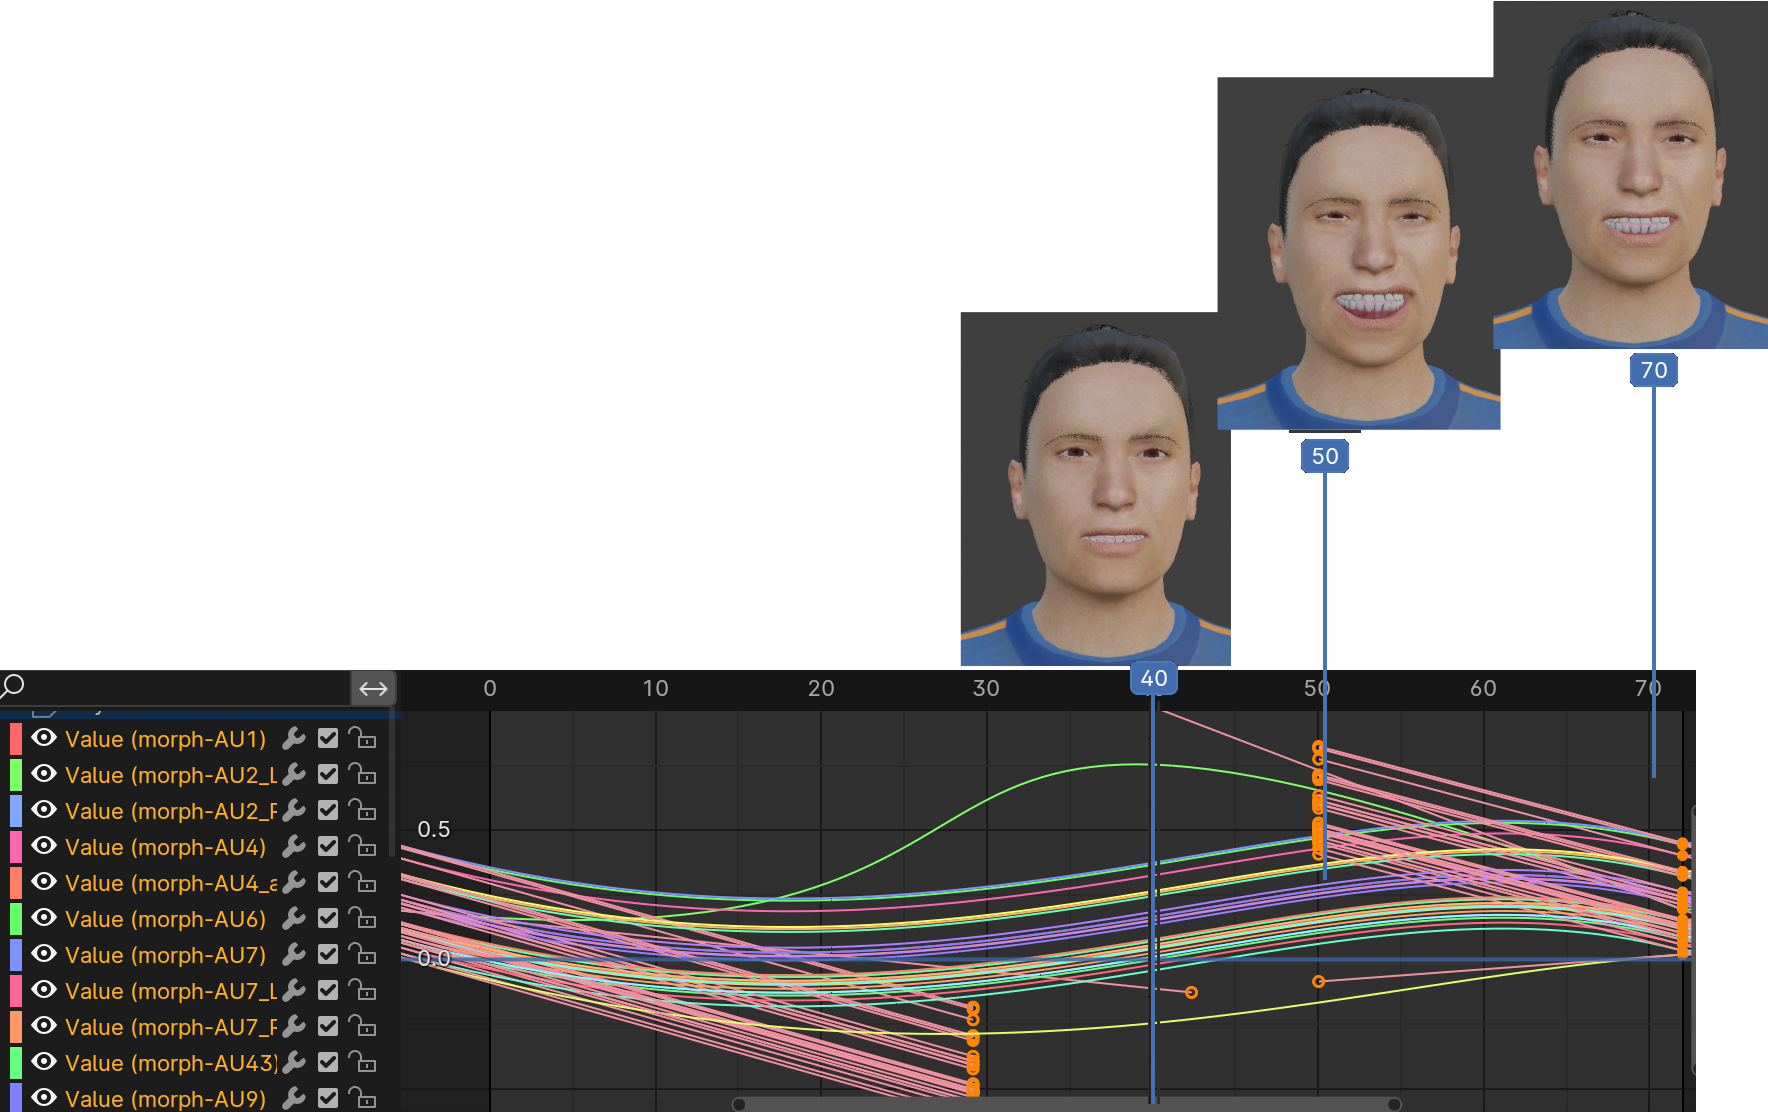
\includegraphics[width = 4in]{chapters/intermediate_blocks_pose_correction/images/motion_curves_shape_keys.png}
    \caption{Motion Curves for \emph{big-threatening}}
    \label{fig:motion_curves_shape_keys}
\end{figure}

After creating the blendshapes, we used motion curve based templates (as discussed earlier in chapter~\ref{ch:intermediate_blocks_pose_correction}) to control how these shapes are animated over time. Motion curves define the changes in the blendshape's influence over the course of an animation, allowing for smooth transitions between different facial expressions.

\begin{figure}[h]
    \centering 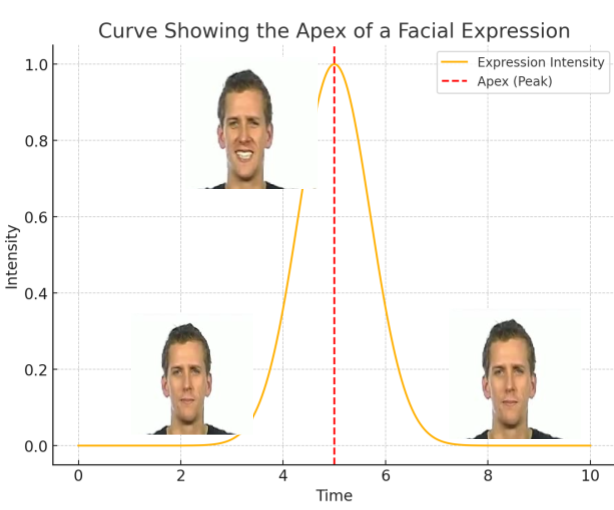
\includegraphics[width = 4in]{chapters/facial_expressions/images/motion_curve_apex.png}
    \caption{Apex of \emph{big-threatening}}
    \label{ch:facial_expressions:fig:motion_curve_apex}
\end{figure}

We used the still images from the corpus as the apex of our curves (figure~\ref{ch:facial_expressions:fig:motion_curve_apex}). Next, we extended our existing intermediate block generation algorithm to include motion curves for facial morphs. This involved creating additional curves that specify the timing and intensity of facial movements based on the template. By controlling the acceleration and deceleration of these movements, we were able to create more naturalistic animations that reflect the dynamic nature of facial expressions.

For example, in the expression \emph{big-threatening}, the motion curves were designed to gradually increase the influence of the blendshapes corresponding to AU10 (Upper Lip Raiser) and AU25 (Lips Part) while simultaneously decreasing the influence of AU4 (Brow Lowerer) as the expression transitions from a neutral state to one of aggression (figure~\ref{fig:motion_curves_shape_keys}).

\section{Results and Evaluation}
\label{ch:facial_expressions:results}

Synthesis of 22 facial expressions from the 40 brèves corpus can be seen in table~\ref{tab:facial_expressions}. The expressions were created by combining the relevant blendshapes to produce realistic and expressive facial animations.

\begin{longtable}{|l|c|r|}
    \caption{Synthesized Expressions} \label{tab:facial_expressions} \\
    \hline
    \textbf{AZee rule} & \textbf{Original Expression} & \textbf{Synthesized Expression} \\
    \hline
    \endfirsthead

    \hline
    \textbf{AZee rule} & \textbf{Original Expression} & \textbf{Synthesized Expression} \\
    \hline
    \endhead

    \hline
    \endfoot

    \hline
    \endlastfoot

    \emph{almost-reaching:} & \includegraphics[width=0.15\textwidth]{chapters/facial_expressions/images/original_facial_expressions/almost_reaching.png} & \includegraphics[width=0.15\textwidth]{chapters/facial_expressions/images/synthesized_expressions/almost_reaching.png} \\
    \emph{big-threatening:} & \includegraphics[width=0.15\textwidth]{chapters/facial_expressions/images/original_facial_expressions/big_threatening.png} & \includegraphics[width=0.15\textwidth]{chapters/facial_expressions/images/synthesized_expressions/big_threatening.png} \\
    \emph{closer-look:} & \includegraphics[width=0.15\textwidth]{chapters/facial_expressions/images/original_facial_expressions/closer_look.png} & \includegraphics[width=0.15\textwidth]{chapters/facial_expressions/images/synthesized_expressions/closer_look.png} \\
    \emph{continuously:} & \includegraphics[width=0.15\textwidth]{chapters/facial_expressions/images/original_facial_expressions/continuously.png} & \includegraphics[width=0.15\textwidth]{chapters/facial_expressions/images/synthesized_expressions/continuously.png} \\
    \emph{do-you-realise:} & \includegraphics[width=0.15\textwidth]{chapters/facial_expressions/images/original_facial_expressions/do_you_realise.png} & \includegraphics[width=0.15\textwidth]{chapters/facial_expressions/images/synthesized_expressions/do_you_realise.png} \\
    \emph{impressive-grandiose:} & \includegraphics[width=0.15\textwidth]{chapters/facial_expressions/images/original_facial_expressions/impressive_grandiose.png} & \includegraphics[width=0.15\textwidth]{chapters/facial_expressions/images/synthesized_expressions/impressive_grandiose.png} \\
    \emph{inter-subjectivity:} & \includegraphics[width=0.15\textwidth]{chapters/facial_expressions/images/original_facial_expressions/inter_subjectivity.png} & \includegraphics[width=0.15\textwidth]{chapters/facial_expressions/images/synthesized_expressions/inter_subjectivity.png} \\
    \emph{it-is-a-shame:} & \includegraphics[width=0.15\textwidth]{chapters/facial_expressions/images/original_facial_expressions/it_is_a_shame.png} & \includegraphics[width=0.15\textwidth]{chapters/facial_expressions/images/synthesized_expressions/it_is_a_shame.png} \\
    \emph{most-probably:} & \includegraphics[width=0.15\textwidth]{chapters/facial_expressions/images/original_facial_expressions/most_probably.png} & \includegraphics[width=0.15\textwidth]{chapters/facial_expressions/images/synthesized_expressions/most_probably.png} \\
    \emph{much-almost-too-much:} & \includegraphics[width=0.15\textwidth]{chapters/facial_expressions/images/original_facial_expressions/much_almost_too_much.png} & \includegraphics[width=0.15\textwidth]{chapters/facial_expressions/images/synthesized_expressions/much_almost_too_much.png} \\
    \emph{nothing-sticks-out:} & \includegraphics[width=0.15\textwidth]{chapters/facial_expressions/images/original_facial_expressions/nothing_sticks_out.png} & \includegraphics[width=0.15\textwidth]{chapters/facial_expressions/images/synthesized_expressions/nothing_sticks_out.png} \\
    \emph{peacefully:} & \includegraphics[width=0.15\textwidth]{chapters/facial_expressions/images/original_facial_expressions/peacefully.png} & \includegraphics[width=0.15\textwidth]{chapters/facial_expressions/images/synthesized_expressions/peacefully.png} \\
    \emph{something-sticks-out:} & 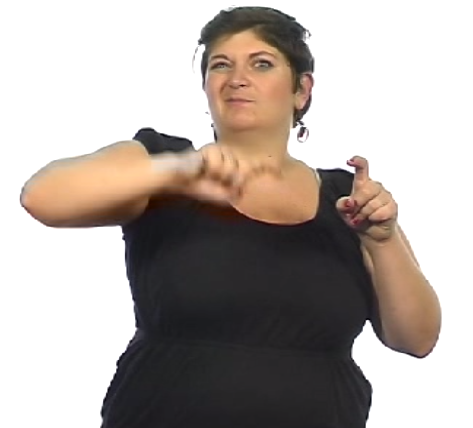
\includegraphics[width=0.15\textwidth]{chapters/facial_expressions/images/original_facial_expressions/sth_sticks_out.png} & 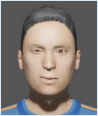
\includegraphics[width=0.15\textwidth]{chapters/facial_expressions/images/synthesized_expressions/something_sticks_out.png} \\
    \emph{takes-a-while:} & \includegraphics[width=0.15\textwidth]{chapters/facial_expressions/images/original_facial_expressions/takes_a_while.png} & \includegraphics[width=0.15\textwidth]{chapters/facial_expressions/images/synthesized_expressions/takes_a_while.png} \\
    \emph{too-scared-to-look:} & \includegraphics[width=0.15\textwidth]{chapters/facial_expressions/images/original_facial_expressions/too_scared_to_look.png} & \includegraphics[width=0.15\textwidth]{chapters/facial_expressions/images/synthesized_expressions/too_scared_to_look.png} \\
    \emph{trouble-disturbance:} & \includegraphics[width=0.15\textwidth]{chapters/facial_expressions/images/original_facial_expressions/trouble_disturbance.png} & \includegraphics[width=0.15\textwidth]{chapters/facial_expressions/images/synthesized_expressions/trouble_disturbance.png} \\
    \emph{uneasy-awkward:} & \includegraphics[width=0.15\textwidth]{chapters/facial_expressions/images/original_facial_expressions/uneasy_awkward.png} & \includegraphics[width=0.15\textwidth]{chapters/facial_expressions/images/synthesized_expressions/uneasy_awkward.png} \\
    \emph{with-chaos:} & \includegraphics[width=0.15\textwidth]{chapters/facial_expressions/images/original_facial_expressions/with_chaos.png} & \includegraphics[width=0.15\textwidth]{chapters/facial_expressions/images/synthesized_expressions/with_chaos.png} \\
    \emph{with-no-precision:} & \includegraphics[width=0.15\textwidth]{chapters/facial_expressions/images/original_facial_expressions/with_no_precision.png} & \includegraphics[width=0.15\textwidth]{chapters/facial_expressions/images/synthesized_expressions/with_no_precision.png} \\
    \emph{with-surprise:} & \includegraphics[width=0.15\textwidth]{chapters/facial_expressions/images/original_facial_expressions/with_surprise.png} & \includegraphics[width=0.15\textwidth]{chapters/facial_expressions/images/synthesized_expressions/with_surprise.png} \\
    \emph{with-uncertainty:} & \includegraphics[width=0.15\textwidth]{chapters/facial_expressions/images/original_facial_expressions/with_uncertainty.png} & \includegraphics[width=0.15\textwidth]{chapters/facial_expressions/images/synthesized_expressions/with_uncertainty.png} \\
    \emph{with-worry:} & \includegraphics[width=0.15\textwidth]{chapters/facial_expressions/images/original_facial_expressions/with_worry.png} & \includegraphics[width=0.15\textwidth]{chapters/facial_expressions/images/synthesized_expressions/with_worry.png} \\
\end{longtable}

Video~\footnote{\url{https://github.com/Paritosh97/phd/raw/master/supplementary_material/ch6allaus.mp4}} shows the range of all the blendshapes in AZee's morph set. Video~\footnote{\url{https://github.com/Paritosh97/phd/raw/master/supplementary_material/ch6allexpressions.mp4}} shows all the synthesized facial expressions with their interpolations.

Table~\ref{tab:facial_expressions_evaluation} shows the subjective evaluation by the linguist who created the corpus of the facial expressions using AZee. The expressions were assessed on isolated still images of the apex of their blendshapes based on their accuracy, expressiveness, and effectiveness in conveying the intended emotional and grammatical cues.

\begin{table*}[h]
    \centering
    \begin{tabular}{|l|p{8cm}|}
    \hline
    \textbf{Expression} & \textbf{Limitations} \\
    \hline
    \texttt{almost-reaching} & Mouth modeling unconvincing. \\
    \hline
    \texttt{continuously} & "Pffff" air and cheek puff difficult, neutral eyebrows. \\
    \hline
    \texttt{do-you-realise} & Thick eyebrow issue. \\
    \hline
    \texttt{it-is-a-shame} & Mouth expression not quite real. \\
    \hline
    \texttt{most-probably} & Less visible teeth preferred, thick eyebrow issue. \\
    \hline
    \texttt{much-almost-too-much} & Frowning eyebrows and lack of eye wrinkles not convincing. \\
    \hline
    \texttt{nothing-sticks-out} & Tucked lips difficult to model. \\
    \hline
   \texttt{something-sticks-out} & Interpreted as confusion, mouth modeling limitation. \\
    \hline
    \texttt{trouble-disturbance} & Frowning eyebrows difficult, mouth "rising" hard to model, result not convincing. \\
    \hline
    \texttt{uneasy-awkward} & Tongue tip out with slightly open mouth hard to model, unconvincing. \\
    \hline
    \texttt{with-chaos} & Single cheek blow/puff and alternating eye blinks hard without animation. \\
    \hline
    \texttt{with-no-precision} & Upper lip over lower and mouth near nose unmodellable. \\
    \hline
    \texttt{with-surprise} & Cannot lower lower eyelid fully, thick eyebrow issue. \\
    \hline
    \texttt{with-uncertainty} & Appears sadder than uncertain, thick eyebrow issue. \\
    \hline
    \texttt{with-worry} & Lack of wrinkles around nose/forehead. \\
    \hline
    \end{tabular}
    \caption{Limitations for the synthesized blendshapes}
    \label{tab:facial_expressions_evaluation}
\end{table*}

We observe that expressions that involved subtle mouth movements, such as "it-is-a-shame" or "something-sticks-out," were more challenging to model accurately, highlighting areas for further refinement.

We also compare the synthesized utterance \emph{big-threatening(hot())} (with facial expressions) and the utterance \emph{hot()} (without facial expressions) to evaluate the impact of facial expressions on \gls{sl} comprehension along with the original video. The results can be seen in the supplementary video\footnote{\url{https://github.com/Paritosh97/phd/raw/master/supplementary_material/ch6_comparison.mp4}}. We observe how non-manuals can enhance the meaning of the sign.

\section{Conclusion}
\label{ch:facial_expressions:conclusion}

% add dynamic morphs curve thing

In this chapter, we presented a method for synthesizing facial expressions using the AZee framework, focusing on the creation of blendshapes from action units (AUs) and the generation of motion curves to control these shapes over time. Our method involved analyzing AUs from the \gls{facs} system and extending the morph set in the AZee language with 94 blendshapes. Next we created those blendshapes on our avatar based on a MakeHuman template mesh. We also used motion curves to animate these blendshapes. The synthesized facial expressions were evaluated subjectively by the linguist who created them. The results show that even though some of the expressions were challenging to model accurately, our method was able to generate some expressions which were effective in conveying the intended form of the corresponding AZee rule.

For future, we plan to use more modern systems to refine the blendshapes and motion curves to improve the accuracy and naturalness of the facial expressions. A good starting point for this would be to animate these rules using a point cloud based capturing systems and then study the capture data to accurately define blendshapes as well as motion templates. Use of emotion recognition systems such as~\cite{danvevcek2022emoca} can be used on the existing dataset to define the flame~\cite{FLAME} principle components. However, establishing a link between the AZee rule and these principle components which drive the mesh will be a challenge. Some synthesized facial expressions using the FLAME model on a default SMPL-X avatar can be seen in the annex section \ref{annex:facial_expressions:flame}.

\end{document}